\begin{center}
 \textsf{Листок 5.}
\end{center}
\vspace{0.01cm}
\nopagebreak[2]
\task{
  Размеры пластин плоского конденсатора увеличили в два раза. Как
  изменилась его ёмкость? Как изменится ёмкость, если расстояние между
  пластинами удвоить? 
}

\task{
  Определите ёмкость конденсатора, образованного двумя
  концентрическими сферами радиуса $R_1$ и $R_2$.
}

\task{ Определите ёмкость систем конденсаторов, изображённых на
  рисунке. На последнем рисунке ёмкости всех конденсаторов равны $C$.}

\task{
  Как изменится ёмкость плоского конденсатора, если поместить его в
  металлическую коробку? Расстояние от обкладок до стенок коробки
  равно расстоянию между обкладками $d$. Как изменится ёмкость, если
  коробку соединить с одной из обкладок? 
}

\begin{figure}[ht]
  \centering
  \subfloat{
    \begin{circuitikz}
      \draw[thick] (0,2) to[capacitor,l=$C_1$] (1.5,2) to[capacitor,l=$C_2$] (3,2);
    \end{circuitikz}}
  \hspace{1cm}
  \subfloat{
    \begin{circuitikz}
      \draw[o-,thick] (0,2) -- (0.5,2) -- (0.5,3);
      \draw[thick] (0.5,2) -- (0.5,1) to[capacitor,l=$C_2$] (2,1) -- (2,3);
      \draw[thick] (0.5,3) to[capacitor,l=$C_1$] (2,3);
      \draw[-o,thick] (2,2) -- (2.5,2);
    \end{circuitikz}}
  \hspace{1cm}
  \subfloat{
    \begin{circuitikz}
      \begin{scope}[thick]
        \draw[o-] (0,2) --++(0.5,0);
        \draw (0.5,2) to[capacitor,l=$C$] (2,3.5) to[capacitor,l=$2C$] (3.5,2)
        to[capacitor,l=$2C$] (2,0.5) to[capacitor,l=$C$] (0.5,2);    
        \draw (2,3.5) to[capacitor,l=$C$] (2,0.5);
        \draw[-o] (3.5,2) -- (4,2);
      \end{scope}
\end{circuitikz}}
\\ \vspace{1cm}
\subfloat{\begin{circuitikz}
  \begin{scope}[thick]
    \draw[o-] (0,3) -- ++(0.5,0);
    \draw (0.5,3) to[capacitor,l=$C$] (1.5,3) to[capacitor,l_=$C$]
    (1.5,1) -- (3,1) to[capacitor,l=$C$] (3,3) to[capacitor,l_=$C$] (1.5,3);
    \draw (3,3) -- (4,3) node[right] {$\ldots$};
    \draw (3,1) -- (4,1) node[right] {$\ldots$};
    \draw[o-] (0,1) -- (1.5,1);
  \end{scope}
\end{circuitikz}}
\hspace{1cm}
\subfloat{
  \begin{circuitikz}
  \begin{scope}[thick]
    \draw[o-] (0,0.5) -- (1,1);
    \draw (1,1) to[capacitor] (1,4) to[capacitor] (4,4) to[capacitor]
    (4,1) to[capacitor] (1,1);
    \draw (4,1) to[capacitor] (6,2) to[capacitor] (6,5) to[capacitor]
    (4,4);
    \draw (6,5) to[capacitor] (3,5) to[capacitor] (1,4);
    \draw[dashed] (3,5) to[capacitor] (3,2) to[capacitor] (6,2);
    \draw[dashed] (1,1) to[capacitor] (3,2);
    \draw[-o] (6,5) -- (7,5.5);
  \end{scope}
\end{circuitikz}}
\caption{К задаче 31.}
\end{figure}


% \begin{center}
% 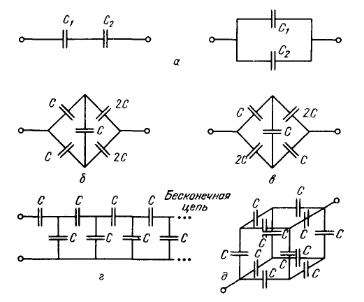
\includegraphics[scale=0.6]{d10_5_1.png}  
% \end{center}

%%% Local Variables: 
%%% mode: latex
%%% TeX-master: "../../../report"
%%% End: 
